% ============================================================
%  深圳大学实验报告模板（SZU Experiment Report Template）
% This template can be modified according to the specific requirements of your experiment or project.
% Produced by: Chao Fan and Kewei Ou, AI School of SZU
% ============================================================

\documentclass[a4paper,12pt]{article}

% ----------------------------
% 中文与字体支持
% ----------------------------
\usepackage{fontspec}    % 字体支持
\usepackage{xeCJK}       % 中文字体支持
\setCJKmainfont{Noto Serif CJK SC} % 设置中文字体（Overleaf自带Noto字体）

% ----------------------------
% 页面设置与常用宏包
% ----------------------------
\usepackage{geometry}    % 页面边距控制
\geometry{left=1in, right=1in, top=1in, bottom=1in}

\usepackage{longtable}   % 支持长表格
\usepackage{graphicx}    % 插入图片
\usepackage{fancyhdr}    % 页眉页脚控制
\usepackage{tikz}        % 绘制框线等图形
\usetikzlibrary{calc}    % 坐标计算
\usepackage{verbatim}    % 显示代码块
\usepackage{float}       % 控制图片浮动位置（[H]参数）

% ----------------------------
% 页眉页脚设置
% ----------------------------
% \pagestyle{fancy}
\fancyhf{} % 清空默认页眉页脚
% \fancyhead[L]{深圳大学实验报告} % 左侧页眉文字
\fancyhead[C]{} % 中间空
\fancyhead[R]{} % 右侧空

% ============================================================
%                      文档开始
% ============================================================

\begin{document}

% ============================================================
% 封面页
% ============================================================
\begin{titlepage}
    \centering
    \vspace*{2cm}
    \Huge{\textbf{深 \ 圳 \ 大 \ 学 \ 实 \ 验  \ 报 \ 告}}\\[1.5cm]

    {\Large\textbf{课程名称}\quad\underline{\makebox[8cm][c]{Python程序设计}}}\\[0.5cm]
{\Large
\noindent\makebox[3.2cm][l]{\textbf{项目名称}}
\underline{\makebox[8cm][c]{基于 NumPy 的 ViT-B/32 图像编码器复现}}}\\[0.5cm]
{\Large
\noindent\makebox[3.2cm][l]{\textbf{学 \quad \quad 院}}
\underline{\makebox[8cm][c]{人工智能学院}}}\\[0.5cm]
{\Large
\noindent\makebox[3.2cm][l]{\textbf{专 \quad \quad 业}}
\underline{\makebox[8cm][c]{人工智能IEEE}}}\\[0.5cm]
{\Large
\noindent\makebox[3.2cm][l]{\textbf{指导教师}}
\underline{\makebox[8cm][c]{舒婷}}}\\[0.5cm]
{\Large
\noindent\makebox[3.2cm][l]{\textbf{报 \quad 告 \quad 人}}
\underline{\makebox[3cm][c]{裴曼秋}}
\hspace{0.5cm}
\textbf{学号}
\underline{\makebox[3cm][c]{2025681082}}}\\[0.5cm]
{\Large
\noindent\makebox[3.2cm][l]{\textbf{实验时间}}
\underline{\makebox[8cm][c]{2026.11.9 - 2026.11.13}}}\\[0.5cm]
{\Large
\noindent\makebox[3.2cm][l]{\textbf{提交时间}}
\underline{\makebox[8cm][c]{2026.11.13}}}\\[1.5cm]

    \vfill
    \Large{\textbf{教务处制}}
\end{titlepage}

\newpage

% ============================================================
% 正文部分
% ============================================================

\section{Objectives 实验目标}

本实验在纯 NumPy 环境下完成，不安装 PyTorch、不联网下载模型、也不进行参数训练。
依据课程提供的已训练权重，复现 OpenCLIP ViT-B/32 图像编码器的前向计算：输入一批
经过预处理的图片，输出每张图一行 512 维、长度归一化的特征向量，并与独立的 FP32
参考结果在数值上对齐。完成后的编码器将作为后续图文匹配 CLIP 大作业的图像塔复用。
此外，配套完成 12 道 NumPy 练习题，巩固数组形状、矩阵运算、汇总与广播等基础操作。

模型固定配置为：输入图像 224$\times$224，patch 大小 32，共 7$\times$7=49 个 patch；
特征宽度 768，12 个注意力头，头维 64，12 层 Transformer Block，MLP 中间宽度 3072，
最终输出维度 512。

% Experiment Process
\section{Overview 方法概述}
整体流程为“切 patch $\rightarrow$ 嵌入编码 $\rightarrow$ 逐层 Transformer 加工
$\rightarrow$ 取 CLS 输出”，如图~\ref{fig:vit-arch} 所示：
\begin{enumerate}
    \item[Spot 1] 图像预处理：等比缩放后中心裁剪到 224$\times$224，按通道均值与方差
    归一化，组织为 batch 数组 $[B,3,224,224]$；
    \item[Spot 2] Patch 嵌入：切分为 7$\times$7=49 个 32$\times$32 方块并展平为 3072 维，
    线性投影到 768 维；前置拼接可学习的 CLS 向量，加入位置编码，得到 $[B,50,768]$；
    \item[Spot 3] Transformer 编码：经 pre-Norm 后通过 12 层 Block（多头注意力加 MLP，
    各带一条残差），取 CLS 行经后归一化、投影到 512 维并单位化，得到 $[B,512]$。
\end{enumerate}

% Figure
\begin{figure}[t]
    \centering
    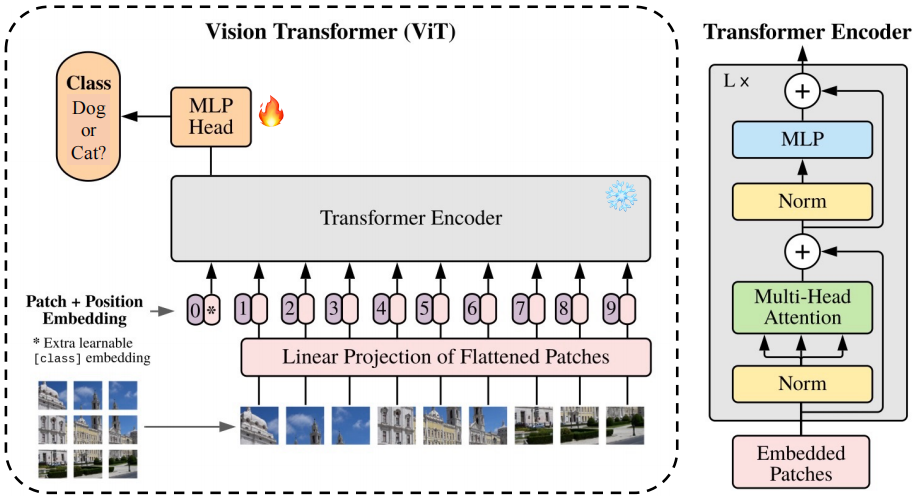
\includegraphics[width=0.92\linewidth]{figs/vit_overview.png}
    \caption{Vision Transformer 整体架构：patch 与位置编码输入 Transformer Encoder，
    最终由 CLS 向量输出特征表示}
    \label{fig:vit-arch}
\end{figure}

% Implementation Details
\section{Implementations 实现细节}
本人贡献：在理解编码器接口与数据流的基础上，补全 \texttt{image\_encoder.py} 中
TODO-02 至 TODO-06 的全部实现；完成 12 道 NumPy 练习题；整理 README 与本报告。
课程提供的预处理、LayerNorm、精确 GELU、注意力 softmax 与单位化工具均未改动。

如图~\ref{fig:vit-arch} 所示，关键实现分为三部分：
\begin{enumerate}
    \item[Part 1] Patch 化与嵌入：\texttt{patchify} 将 $[B,3,224,224]$ 重排为 7$\times$7
    patch 网格并按 C,H,W 顺序展平为 $[B,49,3072]$；patch 投影无 bias，使用
    \texttt{patch\_weight.T} 完成线性变换；前置拼接 CLS 后按行加入位置编码。
    \item[Part 2] 多头注意力与 Block：\texttt{split\_heads} 把 768 维特征 reshape 为
    $[B,N,12,64]$ 再 transpose 为 $[B,12,N,64]$；QK 分数除以 $\sqrt{64}$，softmax 后
    加权 Value，再合并头并输出投影。Block 含两条残差：先加注意力输出，再经 Norm 2、
    GELU 激活的 MLP 后加第二次残差。
    \item[Part 3] 输出头：选取第 0 行 CLS，经 post-Norm 后投影到 512 维；
    \texttt{visual.proj} 已是 [输入, 输出] 布局，不再转置，最后由单位化函数归一化。
\end{enumerate}

权重方向约定：注意力与 MLP 线性权重按 [输出, 输入] 存储，矩阵乘时使用
\texttt{weight.T}；最终投影矩阵除外。关键代码如下：

\begin{verbatim}
# split_heads: [B,N,D] -> [B,H,N,D/H]
x = x.reshape(B, N, self.heads, self.head_dim)
x = x.transpose(0, 2, 1, 3)

# scores: q [B,H,N,64] @ k^T [B,H,64,N] -> [B,H,N,N]
scores = q @ k.swapaxes(-1, -2) / np.sqrt(np.float32(self.head_dim))
\end{verbatim}

\section{Results 结果}

\texttt{check.py} 将实现结果与独立 FP32 参考逐阶段比对，检查形状、float32 类型、
有限值，并按阶段使用绝对误差容忍（atol）与相对误差 rtol=2e-4。八个阶段全部通过，
实测误差如表~\ref{tab:errors}。

\begin{table}[H]
    \centering
    \begin{tabular}{lcccc}
        \hline
        阶段 & 形状 & 最大绝对误差 & 平均绝对误差 & 容忍 atol \\
        \hline
        preprocess   & (10, 3, 224, 224) & 0.000e+00 & 0.000e+00 & 2e-6 \\
        patches      & (2, 49, 3072)     & 0.000e+00 & 0.000e+00 & 2e-4 \\
        tokens       & (2, 50, 768)      & 4.005e-05 & 1.289e-06 & 2e-4 \\
        block0       & (2, 50, 768)      & 7.063e-06 & 3.250e-07 & 2e-4 \\
        last\_tokens & (2, 50, 768)      & 4.768e-05 & 2.696e-06 & 2e-4 \\
        output       & (10, 512)         & 5.439e-07 & 8.311e-08 & 2e-5 \\
        batch        & (3, 512)          & 4.619e-07 & 7.632e-08 & 2e-5 \\
        \hline
    \end{tabular}
    \caption{分阶段数值比对误差}
    \label{tab:errors}
\end{table}

batch 阶段故意打乱图片顺序并重复输入图片，输出仍与参考一致，说明结果来自真实前向
计算，而非写死参考行。\texttt{run.py} 对 10 张图输出形状 (10, 512) 的 float32 向量，
每行长度均为 1。

\section{Discussion 讨论}

\subsection{一个形状变化：注意力分头与合头}
多头注意力需要把 768 维特征平均拆给 12 个头。\texttt{split\_heads} 先 reshape 为
$[B,N,12,64]$，再 \texttt{transpose(0,2,1,3)} 得到 $[B,12,N,64]$；计算完成后按逆
操作转回 $[B,N,12,64]$，再 reshape 合并为 $[B,N,768]$。拆分与合并须保证每个头拿到
连续的 64 维切片，且 token 顺序在前后保持不变。

\subsection{一个修复的 Bug：transpose 不接受负索引}
计算 QK 分数时最初写成 \texttt{k.transpose(-1,-2)} 只交换最后两轴，在 block0 阶段
报错 “axes don't match array”。原因是 NumPy 的 \texttt{transpose} 位置参数只接受
非负轴序号，负索引不会被解析为“倒数第几个轴”。改用
\texttt{k.swapaxes(-1,-2)} 后问题解决：\texttt{swapaxes} 支持负轴，且只交换最后两轴，
保留 batch 与头的分组，分数形状正确得到 $[B,H,N,N]$。

\subsection{不足与改进}
课程提供的 GELU 采用逐值循环调用 \texttt{math.erf}，在批量较大时速度有限；本作业
图片规模较小，精度与速度均可接受，后续可向量化该激活函数以提升效率。

\subsection{所用协助}
实现参考了课程讲义与 \texttt{PPT-CODE-MAP.txt} 的代码—公式对照、
\texttt{transformer\_steps.py} 微型示范、\texttt{helpers.py} 数值工具，以及 NumPy
官方文档；报错定位与形状核对借助 AI 编程助手辅助排查，最终代码、校验结论与练习结果
均由本人在本地运行确认。

\newpage

% ============================================================
% 批阅与成绩评定页
% ============================================================

% 绘制正文外框（包含批阅区域）
\begin{tikzpicture}[remember picture, overlay]
  \draw[thick]
    ($(current page.north west)+(2cm,-3cm)$)
    rectangle
    ($(current page.south east)+(-2cm,3.5cm)$);
\end{tikzpicture}

\vspace{1cm}

% 批阅区
\noindent \textbf{指导教师批阅意见：}
\vspace{6cm}
\hfill

\vspace{1cm}

\noindent \textbf{成绩评定：}
\vspace{2cm}
\hfill

\vspace{1cm}

\noindent
\hfill
\textbf{指导教师签字：}\quad\quad\quad\quad\quad\\[0.5cm]

\hfill
\textbf{年}\quad\quad
\textbf{月}\quad\quad
\textbf{日}\quad

\vspace{1cm}

% 备注部分
\noindent \textbf{备注：}

% 框外的注释
\begin{tikzpicture}[remember picture, overlay]
  \node[
    anchor=north west,
    inner sep=0pt,
    text width=\dimexpr\paperwidth-4cm\relax
  ] at ($(current page.south west)+(2cm,3.1cm)$) {
    \begin{minipage}{\dimexpr\paperwidth-4cm\relax}
      \small
      \noindent
      \textbf{注：}\;1、报告内的项目或内容设置，可根据实际情况加以调整和补充。\\[0.2cm]
      \phantom{\textbf{注：}\;}2、教师批改学生实验报告时间应在学生提交实验报告时间后 10 日内。
    \end{minipage}
  };
\end{tikzpicture}

% ============================================================
%                      文档结束
% ============================================================

\end{document}
